\chapter{Analyse des Besoins et Spécification}

\section*{Introduction du chapitre}
Après avoir décrit le cadre général du projet et analysé le fonctionnement de la solution existante au sein de CIH BANK, ce chapitre se focalise sur la définition claire et rigoureuse des besoins. Nous y détaillons d'une part les besoins fonctionnels, c'est-à-dire les fonctionnalités attendues du pipeline de Data Quality, et d'autre part les besoins non fonctionnels, liés aux exigences techniques, de performance et de sécurité. Enfin, nous présentons la modélisation fonctionnelle à travers la spécification des cas d'utilisation et de leurs acteurs.

% =========================
\section{Besoins fonctionnels}

Les besoins fonctionnels décrivent les actions que le système doit être capable de réaliser pour répondre aux problématiques de qualité des données identifiées sur le domaine Tiers. Ces problématiques, transverses à l'ensemble des tables du référentiel, seront illustrées par la table \texttt{np\_description} et ses 40 colonnes (\texttt{name}, \texttt{firstname}, \texttt{civility}, \texttt{sex}, \texttt{birthdate}, \texttt{nationalitycountry}, \texttt{fatcaidentificationnumber}, etc.). Les besoins se répartissent en quatre fonctionnalités majeures :

\subsection{Automatisation et planification des contrôles}
\begin{itemize}
    \item \textbf{Sous-besoin 1.1 : Déclenchement automatique} : Le système doit lancer l'évaluation de la qualité des données de manière planifiée, immédiatement après l'exécution complète du batch quotidien d'ingestion des tables sources Oracle NOVA (via un nouveau DAG dédié s'exécutant à 00h00, séparé du DAG d'ingestion \texttt{dailyow22} de 22h00) ,
    \item \textbf{Sous-besoin 1.2 : Orchestration intégrée} : L'exécution du scan de qualité doit être orchestrée au sein d'Apache Airflow, permettant de suivre son statut d'exécution (Succès/Échec) et de consulter les logs en temps réel.
\end{itemize}

\subsection{Configuration déclarative des règles de qualité}
\begin{itemize}
    \item \textbf{Sous-besoin 2.1 : Moteur de règles dynamique} : Le système doit permettre de définir les contrôles de qualité (Missing, Invalid, Freshness, Consistency, Uniqueness) dans des fichiers de règles déclaratifs séparés du code source ,
    \item \textbf{Sous-besoin 2.2 : Graduation des seuils et des alertes} : Pour chaque contrôle, le système doit pouvoir évaluer des seuils paramétrables (ex : taux de valeurs manquantes inférieur à 5\%) et générer un statut de warning ou d'error selon la gravité de l'écart ,
    \item \textbf{Sous-besoin 2.3 : Gestion des métadonnées} : Chaque règle doit être documentée avec des attributs métier (nom de la règle, dimension DQ associée, domaine KYC ou CSP, criticité, etc.).
\end{itemize}

\subsection{Historisation et traçabilité des indicateurs}
\begin{itemize}
    \item \textbf{Sous-besoin 3.1 : Persistance journalière} : À chaque exécution, le système doit sauvegarder les métriques calculées et les résultats de chaque contrôle de qualité dans des tables d'historique de scores (base Hive dédiée \texttt{dq\_results}), indexée par date d'exécution ,
    \item \textbf{Sous-besoin 3.2 : Identification des anomalies (Remédiation)} : Le système doit capturer de manière détaillée la liste des enregistrements clients en anomalie en stockant leur identifiant technique (UUID) et leur radical (numéro client), ainsi que le libellé du contrôle en échec et sa criticité. Ces informations doivent être stockées dans une table d'anomalies pour actions correctives.
\end{itemize}

\subsection{Restitution visuelle et aide à la décision}
\begin{itemize}
    \item \textbf{Sous-besoin 4.1 : Exposition des données} : Les résultats d'historisation de la qualité doivent être exposés de manière transparente sous forme de vues SQL pour les outils décisionnels ,
    \item \textbf{Sous-besoin 4.2 : Suivi de l'évolution temporelle} : Le tableau de bord doit permettre de suivre la tendance d'évolution des scores DQ dans le temps (30 derniers jours) ,
    \item \textbf{Sous-besoin 4.3 : Priorisation des remédiations} : Le tableau de bord doit fournir une liste opérationnelle des clients en anomalie triée par criticité décroissante, exportable par les Data Stewards pour traitement correctif dans le système source NOVA.
\end{itemize}

% =========================
\section{Besoins non fonctionnels}

Les besoins non fonctionnels expriment les exigences qualitatives, opérationnelles et techniques que la solution doit respecter pour être viable et performante dans l'environnement de production de CIH BANK :

\subsection{Performance}
Le Référentiel Tiers de la banque regroupe \textbf{plusieurs millions} de dossiers clients (personnes physiques). Les règles de cohérence inter-colonnes ou de doublons nécessitent des jointures lourdes. Le moteur DQ doit être capable d'interroger et d'évaluer ce volume massif de données en un temps minimal (moins de 15 minutes) sans dégrader les ressources du Data Lake. Cela justifie l'utilisation d'un moteur de calcul distribué (Apache Spark) pour le traitement.

\subsection{Disponibilité}
L'exécution des contrôles de qualité ne doit pas bloquer la disponibilité des données pour les outils de reporting en cas d'anomalie. Si un seuil de qualité est franchi ou si le scan échoue, le pipeline d'exposition (Dremio/Tableau) doit continuer à fonctionner en mode dégradé en signalant l'alerte. De plus, la tâche DQ doit s'exécuter même si certaines tables d'ingestion n'ont été chargées que partiellement.

\subsection{Maintenabilité}
L'ajout de nouvelles règles ou l'intégration de nouvelles colonnes du Référentiel Tiers (par exemple pour de nouveaux critères réglementaires ou pour les personnes morales) doit se faire sans modification du code Python principal de la solution. Les fichiers de configuration YAML et la structure des tables Hive de résultats doivent être conçus de manière générique pour supporter l'extensibilité.

\subsection{Sécurité}
Les détails d'anomalies de qualité des données contiennent des informations clients sensibles (\texttt{name}, \texttt{firstname}, radicaux). Seuls les collaborateurs habilités du Data Office (Data Stewards, Data Project) et les Data Owners des départements concernés doivent être autorisés à accéder aux détails des anomalies. La solution s'appuie sur les mécanismes de sécurité existants de la plateforme :
\begin{itemize}
    \item \textbf{Authentification Kerberos} : L'ensemble des composants du cluster Cloudera (HDFS, Hive, Spark) sont sécurisés par Kerberos, garantissant l'identité de chaque service et utilisateur ,
    \item \textbf{Autorisation Apache Ranger} : Les politiques d'accès aux tables Hive et aux espaces HDFS sont gérées de manière centralisée via Ranger, permettant un contrôle fin par rôle ,
    \item \textbf{Annuaire LDAP / Active Directory} : L'authentification des utilisateurs Dremio et Tableau est déléguée à l'annuaire d'entreprise, assurant une gestion unifiée des identités.
\end{itemize}

% =========================
\section{Modélisation des cas d'utilisation}

\subsection{Acteurs du système}
L'intégration de la solution de Data Quality au sein de CIH BANK repose sur une étroite collaboration entre les experts métier, l'équipe technique et les systèmes d'information. Le tableau \ref{tab:acteurs_dq} présente les cinq acteurs clés du système.

\begin{table}[H]
\centering
\caption{Acteurs du système de Data Quality}
\label{tab:acteurs_dq}
\renewcommand{\arraystretch}{1.4}
\resizebox{\textwidth}{!}{
\begin{tabular}{|l|l|p{9cm}|}
\hline
\rowcolor{gray!20}
\textbf{Acteur} & \textbf{Type} & \textbf{Rôle dans le système DQ} \\
\hline
Équipe Data (DE / Data Steward) & Interne & Organise les ateliers d'alignement, formalise les règles dans les fichiers YAML Soda Core et implémente les flux techniques. \\
\hline
Métiers (Data Owners) & Humain & Experts fonctionnels qui définissent et valident les règles de qualité, consultent le dashboard et remédient aux anomalies. \\
\hline
Équipe SI & Appui & Valide la faisabilité technique des règles vis-à-vis du modèle physique Oracle NOVA. \\
\hline
Airflow (Orchestrateur) & Système & Déclenche automatiquement le scan DQ chaque soir après l'ingestion (nouveau DAG à 00h00). \\
\hline
Oracle NOVA (Système source) & Externe & Récepteur final des corrections de données opérées par les gestionnaires suite aux alertes DQ. \\
\hline
\end{tabular}
}
\end{table}

\subsection{Diagramme global des cas d'utilisation}
Le diagramme ci-dessous synthétise graphiquement les cas d'utilisation du système de Data Quality et les interactions avec les différents acteurs impliqués dans ce cycle de gouvernance.

\begin{figure}[H]
\centering
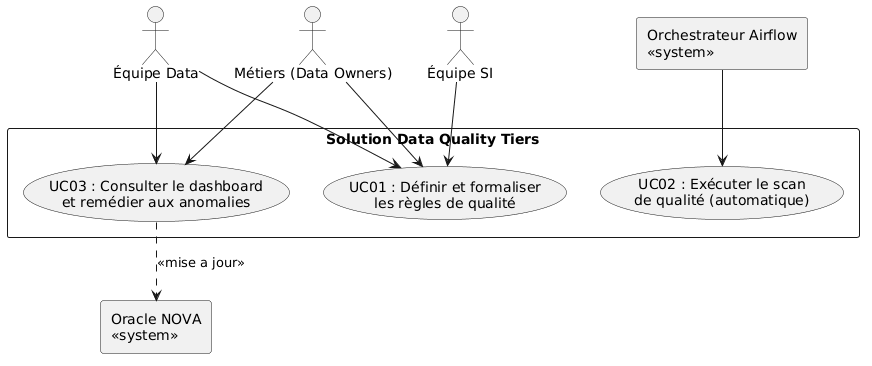
\includegraphics[width=0.95\textwidth]{figures/usecaseGeneral.png}
\caption{Diagramme global des cas d'utilisation de la solution DQ Tiers}
\label{fig:usecase_dq}
\end{figure}

\subsection{Description textuelle des cas d'utilisation principaux}
Nous détaillons ci-dessous le déroulement des trois phases principales constituant le cycle de vie de la qualité des données de notre solution.

\subsubsection{Cas d'utilisation 01 : Définir et formaliser les règles de qualité}

\begin{table}[H]
\centering
\caption{Description du cas d'utilisation 01}
\label{tab:uc01}
\renewcommand{\arraystretch}{1.4}
\begin{tabular}{|l|p{10cm}|}
\hline
\rowcolor{gray!20}
\textbf{Champ} & \textbf{Description} \\
\hline
\textbf{Titre} & Définir et formaliser les règles de qualité \\
\hline
\textbf{Acteurs} & Équipe Data (Steward / DE), Métiers (Data Owners), Équipe SI \\
\hline
\textbf{Préconditions} & Cadrage fonctionnel du domaine Tiers défini \\
\hline
\textbf{Scénario nominal} &
1. L'équipe Data organise des ateliers d'alignement avec les experts Métier et l'équipe SI. \newline
2. Les parties s'accordent sur le catalogue des contrôles (complétude KYC, cohérence CSP) et les seuils de tolérance. \newline
3. L'équipe Data consigne les spécifications dans un document de cadrage. \newline
4. Le Data Engineer implémente les règles dans les fichiers YAML Soda Core. \\
\hline
\textbf{Postconditions} & Les règles de qualité sont formalisées et déployées dans le moteur Soda. \\
\hline
\end{tabular}
\end{table}

\subsubsection{Cas d'utilisation 02 : Exécuter le scan de qualité (automatique)}

\begin{table}[H]
\centering
\caption{Description du cas d'utilisation 02}
\label{tab:uc02}
\renewcommand{\arraystretch}{1.4}
\begin{tabular}{|l|p{10cm}|}
\hline
\rowcolor{gray!20}
\textbf{Champ} & \textbf{Description} \\
\hline
\textbf{Titre} & Exécuter le scan de qualité (automatique) \\
\hline
\textbf{Acteur principal} & Orchestrateur Airflow (Système) \\
\hline
\textbf{Préconditions} & Fin de l'ingestion quotidienne Sqoop des tables NOVA \\
\hline
\textbf{Scénario nominal} &
1. Airflow lance automatiquement la tâche DQ de nuit. \newline
2. Le moteur DQ Soda Core lit les fichiers YAML et exécute les requêtes sur Spark. \newline
3. Les résultats agrégés et les détails des anomalies clients sont historisés dans la base Hive \texttt{dq\_results}. \\
\hline
\textbf{Postconditions} & Les indicateurs et anomalies du jour sont prêts à être exposés. \\
\hline
\end{tabular}
\end{table}

\subsubsection{Cas d'utilisation 03 : Consulter le dashboard et remédier aux anomalies}

\begin{table}[H]
\centering
\caption{Description du cas d'utilisation 03}
\label{tab:uc03}
\renewcommand{\arraystretch}{1.4}
\begin{tabular}{|l|p{10cm}|}
\hline
\rowcolor{gray!20}
\textbf{Champ} & \textbf{Description} \\
\hline
\textbf{Titre} & Consulter le dashboard et remédier aux anomalies \\
\hline
\textbf{Acteurs} & Métiers (Parties prenantes), Data Stewards \\
\hline
\textbf{Préconditions} & Le scan DQ s'est exécuté de manière conforme \\
\hline
\textbf{Scénario nominal} &
1. Le dashboard Tableau se rafraîchit automatiquement chaque matin. \newline
2. Chaque partie prenante consulte le dashboard depuis son poste de travail. \newline
3. Chaque acteur filtre et exporte la liste des anomalies de son périmètre. \newline
4. Les acteurs procèdent à la correction des anomalies dans Oracle NOVA. \\
\hline
\textbf{Postconditions} & Les données corrigées dans NOVA sont ré-ingérées lors du prochain batch et le score DQ s'améliore automatiquement. \\
\hline
\end{tabular}
\end{table}

\section*{Conclusion du chapitre}
Ce chapitre a permis de formaliser les besoins fonctionnels et non fonctionnels, définissant de manière précise les objectifs techniques et opérationnels du pipeline de qualité des données. La modélisation des acteurs et des cas d'utilisation reflète fidèlement le cycle de gouvernance de CIH BANK, où chaque partie prenante collabore d'abord à la définition des contrôles, puis intervient individuellement sur son périmètre pour corriger les anomalies identifiées au quotidien. Fort de ces spécifications, le chapitre suivant présente la conception globale et détaillée de la solution.
